The question of the existence of an analog to bound entanglement was firstly posed in \cite{GisWolf00} by Gisin and Wolf, where they analysed the comparisons and correspondences between quantum and classical protocols for key agreement. 
The rise of bound information was a consequence of these correspondences.\\
Since then the topic was picked up by the scientific community of quantum cryptography and a couple more observation were made.
A probability distribution that presents bound information has not been found yet. Neverthenless 	a case for asymptotic bound information was proposed again by Wolf together with Renner \cite{RW03}.

\section{Tripartite Bound Information}
    %[1]
\section{The gaps between the bounds can be arbitrarily large}
    To distinguish and analyse the case of bound information some information theoretical measures are needed. 
    We already saw the secret key rate (section \ref{seckeyrate}) and the intrinsic information (section \ref{intrininfo}) and we already presented the question of bound information in terms of them. \\
    In \cite{RW03} a new measure of \emph{reduced intrinsic information} is introduced as an upper bound on secret key rate, lower than just the normal intrinsic information.
    For every $P_{XYZ}$ it holds
    \begin{equation}
    	\keyrate{X}{Y}{Z} \leq \redintrinfo{X}{Y}{Z} \leq \intrinfo{X}{Y}{Z}
    \end{equation}
    	Reduced intrinsic information is a strictly stronger upper bound on secret key rate than intrinsic information.
    	More importantly, Renner and Wolf prove that the gap between reduced and normal intrinsic information can be arbitrarily large, implying the existence of asymptotic bound information.
    	\begin{figure}
    		% scheme representing the bounds
% expresed in paper Renner+Wolf 2003
% on the quantities intrinsic information,
% secret key rate and information of formaion

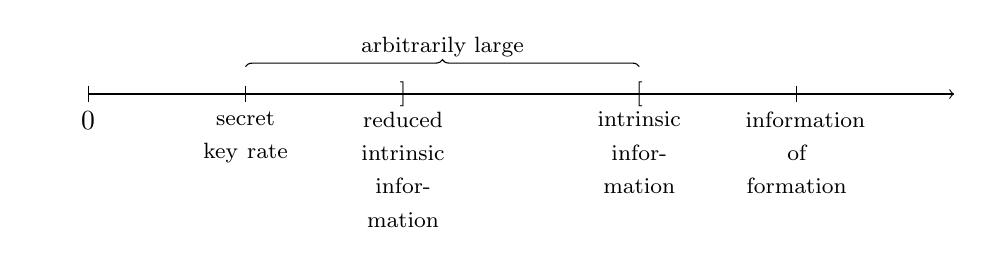
\begin{tikzpicture}

\tikzset{
    position label/.style={
       below = 3pt,
       align=center,
%       text height = 1.5ex,
%       text depth = 1ex,
       text width=13mm
    },
   brace/.style={
     decoration={brace},
     decoration={raise=3ex},
     decorate
   },
   blabel/.style={
		above = 13pt,
		align=center,
		pos=0.5   
   }
}

% draw horizontal line
\draw[->] (0,0) -- (11,0);

%draw vertical lines
\foreach \x in {0,2,9}
   \draw (\x cm,3pt) -- (\x cm,-3pt);
   
\node (foo) at (4cm,0) {\scalebox{0.9}{]}};
\node (bar) at (7cm,0) {\scalebox{0.9}{[}};

%labels
\node [position label] (Start) at (0,0) {$0$};
\node [position label] (skr) at (2,0) {\footnotesize secret key rate};
\node [position label] (rinf) at (4,0) {\footnotesize reduced intrinsic information};
\node [position label] (inf) at (7,0) {\footnotesize intrinsic information};
\node [position label] (iof) at (9,0) {\footnotesize information of formation};

\draw [brace] (skr.north) -- node [blabel] {\footnotesize arbitrarily large} (inf.north);

\end{tikzpicture}
    		\caption{The different measures for $P_{XYZ}$ and how they bound each other.}
    	\end{figure}
\section{A candidate probability distribution}
    Wolf and Renner proposed in \cite{RW03} for the first time a probability distribution which is a good candidate for the classical analogy of \emph{bound entanglement}. 
    In fact, they propose a probability distribution that asymptotically has bound information. 
    They also show, for such a distribution, that $\keyrate{X}{Y}{Z} \neq \intrinfo{X}{Y}{Z}$ and they emphasize that this is the first time that equality does not hold.
	\begin{figure}[h!]
	\begin{center}
		\begin{tabular}{|l r||c|c|c|c|}
		    \hline 
		    		 &	$X$ & $0$ & $1$ & $2$ & $3$ \\ 
		    $Y$ &		  &		&			&			&		\\
		    \hline 
		    \hline
		    $0$ &		   & $1/8$ & $1/8$ & $0$ & $0$ \\ 
		    \hline 
		    $1$ &		   & $1/8$ & $1/8$ & $0$ & $0$ \\ 
		    \hline 
		    $2$ &		   & $0$ & $0$ & $1/4$ & $0$ \\ 
		    \hline 
		    $3$ &		   & $0$ & $0$ & $0$ & $1/4$ \\ 
		    \hline 
		  \end{tabular} 
	\end{center}
		

%\begin{table}[pos]
%\centering
%\caption{My caption}
%\label{my-label}
%\begin{tabular}{|l|l|l|l|l|l|}
%\hline
%\multicolumn{2}{|r|}{$X$} & \multirow{2}{*}{0} & \multirow{2}{*}{1} & \multirow{2}{*}{2} & \multirow{2}{*}{3} \\
%\multicolumn{2}{|l|}{Y}   &                    &                    &                    &                    \\ \hline
%\multicolumn{2}{|l|}{0}   & 1/8                & 1/8                & 0                  & 0                  \\ \hline
%\multicolumn{2}{|l|}{1}   & 1/8                & 1/8                & 0                  & 0                  \\ \hline
%\multicolumn{2}{|l|}{2}   & 0                  & 0                  & 1/4                & 0                  \\ \hline
%\multicolumn{2}{|l|}{3}   & 0                  & 0                  & 0                  & 1/4                \\ \hline
%\end{tabular}
%\end{table}
		
	    $$Z \equiv X + Y\; (mod\: 2)\; \text{ if } X,Y \in \{ 0,1\}$$ 
	    $$Z \equiv X\; (mod\: 2)\; \text{ if } X \in \{ 2,3\}$$ 
	    $$U \equiv \lfloor X/2 \rfloor $$
	    \caption{Probability distribution proposed by Renner, Wolf and Skripsky in \cite{RW03} for which it holds that $\keyrate{X}{Y}{Z} \neq \intrinfo{X}{Y}{Z}$}
	    \label{Tab:candidate}
	\end{figure}	    
	
	\begin{figure}
		\begin{center}
		\begin{tabular}{|l r||c|c|c|c|}
		    \hline 
		    		 &	$X$ & $0$ & $1$ & $2$ & $3$ \\ 
		    $Y$ &		  &		&			&			&		\\
		    \hline 
		    \hline
		    $0$ &		   & $1/8$ & $1/8$ & $a$ & $a$ \\ 
		    \hline 
		    $1$ &		   & $1/8$ & $1/8$ & $a$ & $a$ \\ 
		    \hline 
		    $2$ &		   & $a$ & $a$ & $1/4$ & $0$ \\ 
		    \hline 
		    $3$ &		   & $a$ & $a$ & $0$ & $1/4$ \\ 
		    \hline 
		  \end{tabular} 
	\end{center}
	
			$$Z \equiv X + Y\; (mod\: 2)\; \text{ if } X,Y \in \{ 0,1\}$$ 
	    	$$Z \equiv X\; (mod\: 2)\; \text{ if } X,Y \in \{ 2,3\}$$ 
	    	$$Z = (X,Y) \text{ otherwise} $$
	    	
	    	\caption{A candidate probability distribution for bound information, for $a\geq 0$ (and renormalized).}
	\end{figure}
    